% !TeX spellcheck = pt_PT
\documentclass[11pt,a4paper]{article}
\usepackage{etex}
\reserveinserts{28}

\usepackage[utf8]{inputenc}

\usepackage{hyperref}
\usepackage{amsthm}
\usepackage{amsmath}
\usepackage{amssymb}
\usepackage{amsfonts}
\usepackage[portuguese]{babel}
\usepackage{pictex}
\usepackage[dvips]{graphics}
\usepackage{enumerate}
\usepackage{color}
\usepackage[usenames,dvipsnames]{xcolor}

\usepackage{amsmath}
\usepackage{amssymb}
\usepackage{amsfonts}
\usepackage[portuguese]{babel}
\usepackage{pictex}
\usepackage[dvips]{graphics}
\usepackage{enumerate}
\usepackage{color}
\usepackage{indentfirst}
\usepackage{listings}
\usepackage{tabularx}
\usepackage{multirow}
\usepackage{float}
\usepackage{makeidx}

\usepackage{graphicx}
\setlength{\parindent}{1cm}
\title{\bf{Compiladores - Projecto}\vspace{50mm}\\iJava\vspace{80mm}}
\author{
João Ricardo Lourenço, Nº 2011151194\\
Joaquim Pedro Bento Gonçalves Pratas Leitão, Nº 2011150072}
\makeindex
\begin{document}

\maketitle
\centerline{\textbf{Relatório}}
\pagebreak

\printindex

\renewcommand*\contentsname{Índice}
\tableofcontents

\pagebreak

\section{Introdução}

O presente trabalho pretende-se desenvolver um compilador para a linguagem $iJava$, um pequeno subconjunto da linguagem Java (versão 5.0). Por ser um subconjunto de uma outra linguagem, todos os programas que respeitem as regras impostas em $iJava$ são também, garantidamente, programas válidos em $Java$.

Nesta linguagem todos os programas são constituídos por uma única classe, que possui métodos e atributos estáticos, e públicos. Para além disso, a classe necessita obrigatoriamente de ter um método $main$, onde a execução do programa se inicia. 

Podemos utilizar literais dos tipos inteiro e booleano e variáveis inteiras, booleanas e arrays uni-dimensionais de inteiros e booleanos.

A linguagem implementa também expressões aritméticas e lógicas, operações relacionais simples, instruções de atribuição e controlo ($if-else$ e $while$).

Os métodos definidos, e os respetivos valores de retorno, podem podem ser de qualquer tipo acima mencionado, com exceção do método $main$, que tal como em $Java$ possui como tipo de retorno o tipo $void$.

É também possível passar parâmetros (literais inteiros) ao nosso programa através da linha de comandos. É o método $main$ que vai receber esses parâmetros, armazenando-os num array de objetos do tipo $String$. Embora este tipo de dados não esteja incluído na lista de tipos permitidos em $iJava$, a sua utilização apenas é permitida no método $main$, com a mera finalidade de obter os parâmetros passados ao programa aquando da sua invocação.

O desenvolvimento do compilador foi dividido em três fases distintas.

Numa primeira fase foi realizada a \emph{Análise Lexical} do programa fonte, onde são identificados \emph{tokens}, isto é, cadeias pertencentes à linguagem e que têm significado e relevância para o programa.

Seguiram-se a realização da \emph{Análise Sintática} e \emph{Análise Semântica}, compostas por quatro etapas principais:

\begin{itemize}
\item \textbf{Tradução da gramática-fonte} (fornecida em notação $EBNF$) para o yacc e realização da \textbf{Análise Sintática} do programa, permitindo assim reconhecer se as sequências de \emph{tokens} que o constituem pertencem à linguagem, permitindo-nos assim detetar eventuais erros de sintaxe.

\item \textbf{Construção da árvore de sintaxe abstrata}, etapa realizada em simultâneo com a \textbf{Análise Sintática}. A árvore de sintaxe abstrata irá representar o nosso programa a compilar, recorrendo a uma estrutura em árvore para representar as estruturas sintáticas das cadeias que o constituem.

\item \textbf{Construção da tabela de símbolos}, utilizadas para armazenar informações relevantes sobre a classe (seus atributos e métodos), bem como sobre cada método definido pelo programador (como, por exemplo, o tipo de retorno e os argumentos).

\item \textbf{Verificação de erros semânticos}, etapa principal da \textbf{Análise} \\* \textbf{Semântica}, onde são realizadas verificações de tipos, garantindo que para cada operação a realizar não existem incompatibilidades de tipos entre os operandos nela envolvidos.

\end{itemize}

A última fase do trabalho consistiu na \emph{Geração de Código Intermédio}, da qual resulta, na representação intermédia de \emph{LLVM}, um programa equivalente ao que pretendemos compilar.

FIXME: METER IMAGEM BONITINHA, TIPO CACEIRO???

\pagebreak

\section{Análise Lexical}

Tal como referimos anteriormente, na \emph{Análise Lexical} procedemos à identificação dos \emph{tokens} da nossa linguagem. Para isso utilizámos a ferramenta $lex$, responsável por gerar analisadores lexicais para linguagens.

Assim, no nosso analisador, sempre que é detetada a presença de um comentário no programa a compilar, seja do tipo $// ...$ (comentários de apenas uma linha) ou do tipo $/* ... */$ (comentários multi-linha), os caracteres incluídos nesse comentário são ignorados.

Sempre que é detetado um caracter, ou uma sequência de caracteres, que não constitui nenhum \emph{token} é detetado um erro lexical, sendo impressa uma mensagem de erro, indicando a existência de um caracter ilegal, juntamente com a sua posição no programa.

Adicionalmente, caso se verifique a ocorrência de um comentário multi-linha que não foi devidamente terminado, o erro lexical é também detetado, sendo impressa uma mensagem de erro que indica a posição no programa onde o comentário foi iniciado.

	\subsection{Tokens}

	Em seguida, apresentamos a lista dos \emph{tokens} válidos na linguagem $iJava$ e a lista dos \emph{tokens} reservados que, por essa razão, não estão disponíveis na nossa linguagem:
	
	\begin{itemize}
	\item \textbf{ID}: Sequências alfanuméricas (maiúsculas e minúsculas) começadas por uma letra, podendo conter também símbolos como $"\_"$ e $"\$"$. Este \emph{token} pode também ser descrito na forma da sua expressão regular: \emph{{letra}({letra}|{[0-9]})*}, sendo o \emph{token} \textbf{letra} da nossa autoria, definido por: $[a-z] \mid [A-Z] \mid "\_"|"\$"$
	
	\item \textbf{INTLIT}: Sequências de dígitos decimais e hexadecimais (incluindo a-f e A-F) precedidas de $0x$. Este \emph{token} pode também ser descrito na forma da seguinte expressão regular: \emph{{[0-9]}+|0x[0-9a-fA-F]+}
	
	\item \textbf{BOOLLIT}: $true \mid false$
	
	\item \textbf{INT}: $int$
	
	\item \textbf{BOOL}: $boolean$
	
	\item \textbf{NEW}: $new$
	
	\item \textbf{IF}: $if$
	
	\item \textbf{ELSE}: $else$
	
	\item \textbf{WHILE}: $while$
	
	\item \textbf{PRINT}: $System.out.println$
	
	\item \textbf{PARSEINT}: $Integer.parseInt$
	
	\item \textbf{CLASS}: $class$
	
	\item \textbf{PUBLIC}: $public$
	
	\item \textbf{STATIC}: $static$
	
	\item \textbf{VOID}: $void$
	
	\item \textbf{STRING}: $String$
	
	\item \textbf{DOTLENGTH}: $.length$
	
	\item \textbf{RETURN}: $return$
	
	\item \textbf{OCURV}: $($
	
	\item \textbf{CCURV}: $)$
	
	\item \textbf{OBRACE}: $\{$
	
	\item \textbf{CBRACE}: $\}$
	
	\item \textbf{OSQUARE}: $[$
	
	\item \textbf{CSQUARE}: $]$
	
	\item \textbf{OP1}: $\&\& \mid \mid \mid$
	
	\item \textbf{OP2}: $< \mid > \mid == \mid != \mid <= \mid >=$
	
	\item \textbf{OP3}: $"+" \mid "-"$
	
	\item \textbf{OP4}: $"*" \mid "/" \mid "\%"$
	
	\item \textbf{NOT}: $"!"$
	
	\item \textbf{ASSIGN}: $"="$
	
	\item \textbf{SEMIC}: $";"$
	
	\item \textbf{COMMA}: $","$
	
	\item \textbf{RESERVED}: $abstract \mid continue \mid for \mid switch \mid assert \mid default \mid goto \mid package \mid synchronized \mid do \mid private \mid this \mid break \mid double \mid implements \mid protected \mid throw \mid byte \mid import \mid throws \mid case \mid enum \mid instanceof \mid transient \mid catch \mid extends \mid short \mid try \mid char \mid final \mid interface \mid finally \mid long \mid strictfp \mid volatile \mid const \mid float \mid native \mid super \mid null \mid ++ \mid --$
	\end{itemize}

	Para além dos \emph{tokens} apresentados, definimos outros \emph{tokens}, que passamos a especificar:
	
	\begin{itemize}
	\item \textbf{NEWLINE}: $Token$ correspondente ao caracter de mudança de linha, $\setminus n$
	
	\item \textbf{WHITESPACE}:$Token$ correspondente ao caracter de espaço em branco
	
	\item \textbf{OPEN\_COMMENT}:  $Token$ correspondente ao início de um comentário multi-linha, $/*$
	
	\item \textbf{CLOSE\_COMMENT}: $Token$ correspondente ao fecho de um comentário multi-linha, $*/$
	
	\item \textbf{SINGLE\_LINE\_COMMENT}: $Token$ utilizado para detetar a \\* ocorrência de um comentário de uma linha apenas
	\end{itemize}
	
	Quando implementámos a \emph{Análise Sintática}, para resolver problemas de ambiguidade da gramática foi necessário, entre outras ações que iremos abordar na próxima secção, separar os \emph{tokens} \textbf{OP1}, \textbf{OP2}, \textbf{OP3} e \textbf{OP4} nas diferentes sequências alfanuméricas que os constituíam. Assim, temos ainda os seguintes \emph{tokens}:
	
	\begin{itemize}
	\item \textbf{AND} ("\&\&") e \textbf{OR} ("$||$"), originados a partir do \emph{token} \textbf{OP1}
	
	\item \textbf{LE} ("<"), \textbf{GE} (">"), \textbf{EQ} ("=="), \textbf{NEQ} ("!="), \textbf{LEQ} ("<=") e \textbf{GEQ} (">="), originados a partir do \emph{token} \textbf{OP2}
	
	\item \textbf{PLUS} ("+") e \textbf {MINUS} ("-"), originados a partide do \emph{token} \textbf{OP3}
	
	\item \textbf{MULT} ("*"), \textbf{DIV} ("/") e \textbf{MOD} ("\%"), originados a partir do \emph{token} \textbf{OP4}
	\end{itemize}
	
	\subsection{Comentários}
	
	Para identificarmos a ocorrência de comentários nos programas a compilar recorremos aos \emph{tokens} \emph{OPEN\_COMMENT}, \emph{CLOSE\_COMMENT} e \\* \emph{SINGLE\_LINE\_COMMENT}.
	
	Quando detetamos o \emph{token OPEN\_COMMENT} é criado um novo estado no analisador, que indica a existência de um comentário multi-linha. A esse estamos demos o nome \emph{MULTI\_LINE\_COMMENT\_S}.
	
	Uma vez neste estado, todos os caracteres e \emph{tokens} identificados são ignorados, com exceção do \emph{token} de fecho do comentário multi-linha \\* (\emph{CLOSE\_COMMENT}) e do \emph{token} de fim do ficheiro, $<<EOF>>$, disponível na ferramenta utilizada para desenvolver o analisador (\emph{lex}).
	
	Caso seja identificado o \emph{token CLOSE\_COMMENT}, o estado do analisador é reposto, passando este a ter o seu estado por defeito.
	
	Por outro lado, se for detetado $<<EOF>>$ temos uma situação em que um comentário multi-linha não foi devidamente terminado, pelo que é gerado um erro lexical, terminando a execução do analisador e sendo o utilizador informado da ocorrência do erro e da localização no programa fornecido do comando que inicia o comentário.
	
	Se, por alguma razão, o \emph{token CLOSE\_COMMENT} for identificado quando o analisador não se encontra no estado \emph{MULTI\_LINE\_COMMENT\_S} é detetada a ocorrência de um erro lexical, uma vez que na nossa linguagem não é possível a existência do comando \emph{*/} sem que antes tenha sido colocado um \emph{/*}. Mais uma vez, assim que o erro lexical é detetado o utilizador é informado com uma mensagem que indica a posição no programa onde se deu o erro, e o analisador termina a sua execução.
	
	Ao detetarmos o \emph{token SINGLE\_LINE\_COMMENT} vamos ignorar todos os caracteres e \emph{tokens} que se lhe seguirem, até que seja reconhecido o \emph{token} de mudança de linha (\emph{NEWLINE}). Desta forma estamos a descartar toda a restante linha do programa, após a ocorrência de $\setminus \setminus$, tal como seria desejado proceder no tratamento de comentários de uma linha apenas.
	
	\subsection{Tratamento de Erros Lexicais}
	
	Tal como referimos nos pontos anteriores, sempre que o analisador desenvolvido deteta a ocorrência de um erro lexical (seja por existência de um \emph{token} não permitido ou por não término de um comentário multi-linha), é impressa uma mensagem de erro que indica a posição do erro no programa a compilar (indicando a linha e coluna onde o erro ocorreu).
	
	Quando é detetado um caracter ilegal, o analisador imprime a mensagem de erro, prosseguindo a sua execução na linha seguinte do programa a compilar até ser lido todo o conteúdo do programa.
	
	Tendo sido detetada a ocorrência de um ou mais erros lexicais, após ler todo o programa, o analisador termina a sua execução, não sendo realizado mais nenhum passo da compilação.


\pagebreak

\section{Análise Sintática}

A Análise Lexical permite-nos identificar os \emph{tokens} da linguagem, isto é, os seus "átomos". No entanto, interessa-nos garantir que os \emph{tokens} identificados estão organizados de acordo com a estrutura sintática da linguagem.

Para validar essa organização dos \emph{tokens} necessitamos de utilizar uma gramática, que nos indica como devem estar organizados sintaticamente os \emph{tokens} da linguagem. Para além disso, utilizámos a ferramenta \emph{YACC (Yet Another Compiler Compiler)}, um gerador de analisadores sintáticos.

Assim, utilizamos o analisador lexical (\emph{lex}) desenvolvido para reconhecer os \emph{tokens} da linguagem, que são transferidos para o \emph{yacc} onde, com base na gramática da linguagem fornecida, podemos verificar se o programa a compilar se encontra organizado de acordo com a estrutura sintática da linguagem.

No analisador sintático foi criada uma \emph{union}, que define a estrutura de uma variável \emph{yylval}, utilizada na comunicação entre o \emph{yacc} e o \emph{lex}. Apresentamos desde já a estrutura da \emph{union} criada:

\begin{lstlisting}
%union
{
    char* token;    
    struct _node_t* node;
    int type;
}
\end{lstlisting}

Os \emph{token} detetados no \emph{lex} são comunicados ao analisador sintático através do campo \emph{token} da variável \emph{yylval}.

Para além disso, no analisador sintático definimos ainda três variáveis externas, para uso partilhado entre o \emph{lex} e o \emph{yacc}: Duas do tipo inteiro, \emph{prev\_col} e \emph{prev\_line}, e uma do tipo array de caracteres (\emph{char*}), chamada \emph{yytext} e que contém a cadeia de caracteres lida pelo analisador, em cada momento.

Tal como o nome pode sugerir, \emph{prev\_col} e \emph{prev\_line} são utilizadas para armazenar o valor da coluna e linha (do programa a compilar) analisadas na iteração anterior da execução do analisador. A justificação para essa prende-se com as situações onde ocorrem erros sintáticos, sendo necessário informar o utilizador da localização no programa desse erro.

\begin{figure}[H]
  \centering
      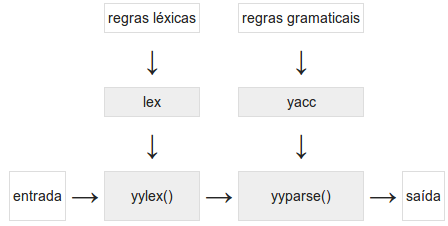
\includegraphics[scale=0.5]{DiagramaLExYACC.png}
  \caption{Ligação entre o \emph{lex} e o \emph{yacc}, ferramentas utilizadas para gerar os analisadores lexicais e sintáticos. Retirado de \emph{http://pt.wikipedia.org/wiki/Yacc}}
\end{figure}

\subsection{Gramática}

De seguida, apresentamos a gramática da linguagem \emph{iJava}, fornecida no enunciado do projeto, em notação \textbf{EBNF}:

\vspace{0.5cm}

\hspace{-1cm}Start $\rightarrow$ Program

\hspace{-1cm}Program $\rightarrow$ CLASS ID OBRACE \{ FieldDecl $\mid$ MethodDecl \} CBRACE

\hspace{-1cm}FieldDecl $\rightarrow$ STATIC VarDecl

\hspace{-1cm}MethodDecl $\rightarrow$ PUBLIC STATIC ( Type $\mid$ VOID ) ID OCURV

\hspace{-.5cm}[ FormalParams ] CCURV OBRACE \{ VarDecl \} \{ Statement \} CBRACE

\hspace{-1cm}FormalParams $\rightarrow$ Type ID \{ COMMA Type ID \}

\hspace{-1cm}FormalParams $\rightarrow$ STRING OSQUARE CSQUARE ID

\hspace{-1cm}VarDecl $\rightarrow$ Type ID \{ COMMA ID \} SEMIC

\hspace{-1cm}Type $\rightarrow$ ( INT $\mid$ BOOL ) [ OSQUARE CSQUARE ]

\hspace{-1cm}Statement $\rightarrow$ OBRACE \{ Statement \} CBRACE

\hspace{-1cm}Statement $\rightarrow$ IF OCURV Expr CCURV Statement [ ELSE Statement ]

\hspace{-1cm}Statement $\rightarrow$ WHILE OCURV Expr CCURV Statement

\hspace{-1cm}Statement $\rightarrow$ PRINT OCURV Expr CCURV SEMIC

\hspace{-1cm}Statement $\rightarrow$ ID [ OSQUARE Expr CSQUARE ] ASSIGN Expr SEMIC

\hspace{-1cm}Statement $\rightarrow$ RETURN [ Expr ] SEMIC

\hspace{-1cm}Expr $\rightarrow$ Expr ( OP1 $\mid$ OP2 $\mid$ OP3 $\mid$ OP4 ) Expr

\hspace{-1cm}Expr $\rightarrow$ Expr OSQUARE Expr CSQUARE

\hspace{-1cm}Expr $\rightarrow$ ID $\mid$ INTLIT $\mid$ BOOLLIT

\hspace{-1cm}Expr $\rightarrow$ NEW ( INT $\mid$ BOOL ) OSQUARE Expr CSQUARE

\hspace{-1cm}Expr $\rightarrow$ OCURV Expr CCURV

\hspace{-1cm}Expr $\rightarrow$ Expr DOTLENGTH $\mid$ ( OP3 $\mid$ NOT ) Expr

\hspace{-1cm}Expr $\rightarrow$ PARSEINT OCURV ID OSQUARE Expr CSQUARE CCURV

\hspace{-1cm}Expr $\rightarrow$ ID OCURV [ Args ] CCURV

\hspace{-1cm}Args $\rightarrow$ Expr \{ COMMA Expr \}

\vspace{0.5cm}

Lembramos que, em notação \textbf{ENBF}, os símbolos \textbf{[...]} englobam \emph{tokens} opcionais e \textbf{\{...\}} implicam a repetição dos \emph{tokens} 0 ou mais vezes.

\subsubsection{Ambiguidade}

Um análise mais cuidada da gramática apresentada permite-nos aferir da sua ambiguidade. Por exemplo, se num dado momento da análise sintática pretendermos analisar $2+3*5$, podemos reduzir esta expressão à variável \emph{EXPR} da gramática por duas formas distintas:

\begin{enumerate}
\item Numa primeira abordagem podemos separar a expressão em \textbf{Expr $\rightarrow$ Expr + Expr} (onde o símbolo \emph{"+"} é proveniente do \emph{token} \emph{OP3}). De seguida reduziríamos o primeiro símbolo \emph{Expr} para o \emph{token} \emph{INTLIT} correspondente, neste caso, ao literal \emph{"2"}. O segundo símbolo \emph{Expr} seria desdobrado em \textbf{Expr $\rightarrow$ Expr * Expr} (onde o símbolo \emph{"*"} é proveniente do \emph{token} \emph{OP4}). Neste caso os dois símbolos \emph{Expr} seriam reduzidos ao \emph{token} \emph{INTLIT}, correspondente a cada um dos restantes literais.

\item Numa abordagem alternativa começaríamos por separar a expressão em \textbf{Expr $\rightarrow$ Expr * Expr}. De seguida desdobraríamos o primeiro símbolo \emph{Expr} em \textbf{Expr $\rightarrow$ Expr + Expr}. Estes dois novos símbolos \emph{Expr} seriam reduzidos a \emph{INTLIT}, tal como o restante símbolo \emph{Expr}.
\end{enumerate}

Acabámos de provar a ambiguidade da gramática. Tal como esta situação existem muitas outras envolvendo os operadores englobados pelos \emph{tokens} \emph{OP1, OP2, OP3 e OP4}. Assim, é imperativa a definição de prioridades nos operadores, de forma a eliminar todas as ambiguidades presentes na gramática, permitindo assim a correta realização da análise sintática do programa.

\subsection{Alterações à Gramática Fornecida}

Uma vez que a gramática apresentada é ambígua e apresenta-se em notação \textbf{EBNF}, não aceite pela ferramenta utilizada para gerar o analisador sintático, necessitamos de alterar a gramática, de forma a eliminar as suas ambiguidades, tornando-a numa gramática aceite pela ferramenta utilizada.

\subsubsection{Definição de Novos \emph{Tokens}}

Como já referimos, a primeira alteração realizada prende-se com a separação dos operadores englobados pelos \emph{tokens} \emph{OP1, OP2, OP3 e OP4}, criando um novo \emph{token} para cada operador, definindo de seguida a prioridade dos diferentes operadores representados pelos \emph{tokens} criados.

As prioridades dos operadores foram definidas na ferramenta \emph{yacc}, de acordo com a sua notação. De seguida apresentamos a definição, em notação \emph{yacc} da prioridade dos operadores identificados:

\begin{lstlisting}
%nonassoc THEN
%nonassoc ELSE
%nonassoc REDUCEEXPRESSON1
%left OR
%left AND
%left EQ NEQ
%left LE GE LEQ GEQ
%left PLUS MINUS
%left MULT DIV MOD
%right ASSIGN
%left OBRACE
%right UNARY_HIGHEST_VAL
%left OSQUARE DOTLENGTH
\end{lstlisting}

\vspace{0.5cm}

Na notação \emph{yacc} a prioridade de um \emph{token} é definida com as instruções \emph{\%left} e \emph{\%right}, correspondendo respetivamente à associatividade à esquerda ou à direita. Alternativamente podemos também utilizar a instrução \emph{\%nonassoc}, indicando que o operador não tem qualquer associatividade. Para além disso a prioridade de um operador é tanto maior quanto posterior for a sua definição.

Na situação apresentada indicamos, por exemplo, que os operadores \emph{THEN} e \emph{ELSE} não têm qualquer associatividade, tendo o operador \emph{ELSE} maior prioridade do que o operador \emph{THEN}.

\subsubsection{Alterações nas Regras da Gramática}

Após a criação de novos \emph{tokens} e definição das respetivas prioridades procedemos a modificações na gramática, visando:

\begin{itemize}
\item Lidar com situações como \emph{Expr $\rightarrow$ ID OCURV [ Args ] CCURV} ou \emph{Args $\rightarrow$ Expr \{ COMMA Expr \}}, correspondentes a \emph{tokens} opcionais e a 0 ou mais repetições de uma dada sequência de \emph{tokens}

\item Distinguir expressões indexáveis, isto é às quais podemos aplicar o operador \textbf{``["}, das restantes operações não indexáveis
\end{itemize}

\subsubsection{\emph{Tokens} Opcionais}

Estas alterações justificam-se pelo facto de que, evitando a existência de símbolos anuláveis, a criação da \emph{Árvore de Sintaxe Abstrata} se tornar mais fácil, dado que as regras anuláveis implicam a criação de nós nulos na \emph{Árvore de Sintaxe Abstrata}, o que adiciona alguma complexidade e dificuldade à sua criação, manutenção e utilização. Por essa razão, e com o principal objetivo de não adicionar demasiada complexidade à criação da \emph{Árvore de Sintaxe Abstrata}, optámos por eliminar essas situações, sempre que possível.

Assim, as situações correspondentes a \emph{tokens} opcionais na gramática foram substituídas pelas respetivas regras, com e sem os \emph{tokens} opcionais. No exemplo apresentado, a regra \emph{Expr $\rightarrow$ ID OCURV [ Args ] CCURV} seria substituída pelas regras \emph{Expr $\rightarrow$ ID OCURV CCURV} e \emph{Expr $\rightarrow$ ID OCURV Args CCURV}.

Por sua vez, as repetições de \emph{tokens} 0 ou mais vezes obrigaram-nos a introduzir um novo símbolo na gramática, que garante a ocorrência da repetição de \emph{tokens} pelo menos uma vez, ou obrigando a que os \emph{tokens} não sejam derivados a partir do símbolo da gramática em questão

Assim, no caso apresentado anteriormente, correspondente à regra \emph{Args $\rightarrow$ Expr \{ COMMA Expr \}}, introduzimos o símbolo \emph{RealArguments}, substituindo a regra por \emph{Args $\rightarrow$ RealArguments}. Por sua vez, o símbolo \emph{RealArguments} possui duas regras, sendo que numa considera apenas uma ocorrência de \emph{Expr} (não ocorrendo nenhuma repetição de \emph{COMMA Expr}), e na outra obriga a que a sequência de \emph{tokens} \emph{COMMA Expr} ocorra pelo menos uma vez. Assim, introduzimos as regras:

\emph{Args $\rightarrow$ RealArguments}
\emph{RealArguments $\rightarrow$ Expr}
\emph{RealArguments $\rightarrow$ Expr COMMA RealArguments}

FIXME: EXPLICAÇÂO BUE MERDOSA. MAXI VE ISTO E DIZ DE TUA JUSTIÇA!!!!!

\subsubsection{Expressões Indexáveis}

À semelhança do que acontece em \emph{Java}, também em \emph{iJava} existem expressões passíveis de serem indexadas e outras onde a operação de indexação não é possível. De seguida apresentamos uma lista das operações indexáveis e não-indexáveis em \emph{iJava}:

\begin{itemize}
\item \textbf{Operações Não-Indexáveis:} Declarações de arrays (inteiros e booleanos), expressões compostas apenas por símbolos terminais (literais inteiros ou booleanos) e expressões onde já é realizada indexação (ou seja, indexáveis)

\item \textbf{Expressões Indexáveis:} Todas as restantes
\end{itemize}

\subsubsection{Expressões Não-Indexáveis}

Dadas as características da linguagem descritas em secções anteriores, uma vez que em \emph{iJava} apenas está disponível a utilização de arrays uni-dimensionais, não podemos considerar as declarações de arrays indexáveis. Caso o fizéssemos, a operação \emph{new int[5][2]} seria válida na nossa linguagem.

De facto, poderíamos entender esta instrução como a declaração de um array uni-dimensional de inteiros, e o posterior acesso à sua terceira posição. No entanto, esta operação corresponde, na linguagem \emph{Java} à declaração de um array bi-dimensional de inteiros, não permitido em \emph{iJava}.

Assim, consideramos a operação \emph{new int[5][2]} inválida na linguagem \emph{iJava}, o que nos permite concluir que todas as declarações de arrays não são indexáveis. Para além disso, caso um programador pretenda declarar um array uni-dimensional e aceder de seguida a uma das suas posições, na mesma linha de código, também o poderá fazer em \emph{iJava}, devendo envolver a declaração do array numa expressão indexável, através da utilização de parêntesis: emph{(new int[5])[2]}.

Pela mesma razão, somos obrigados a considerar expressões onde já é feita indexação (como por exemplo \emph{a[2]}, onde \emph{a} corresponde a um array uni-dimensional de inteiros ou booleanos) como sendo expressões não-indexáveis. Caso contrário operações como \emph{a[2][0]} seriam permitidas, implicando que \emph{a} fosse duplamente indexável. Ou seja, \emph{a} seria um array bi-dimensional, estrutura de dados não permitida na nossa linguagem.


\subsubsection{Expressões Indexáveis}

Todas as expressões que não declarações de arrays ou terminais são passíveis de serem indexadas na nossa linguagem.

Queremos, contudo, chamar a atenção para situações não permitidas na linguagem, como por exemplo \emph{a[0]} caso \emph{a} seja uma variável do tipo inteiro ou booleano.

De facto, a nível sintático esta expressão é considerada válida, sendo apenas na \emph{Análise Semântica} (a detalhar mais à frente) realizadas verificações dos tipos de dados envolvidos em cada operação, assegurando a adequação dos mesmos à operações a realizar. Naturalmente que o exemplo descrito levará à deteção de um erro semântico, que será posteriormente relatado ao utilizador.

\subsubsection{Gramática Final}

Apresentamos de seguida a gramática final da linguagem, após efetuar todas as alterações referidas:

\begin{lstlisting}
Start:	Program
	;

Program: CLASS ID OBRACE Declarations CBRACE
    |    CLASS ID OBRACE CBRACE
	;

Declarations: Declarations FieldDecl
    |     Declarations MethodDecl
    |     FieldDecl
    |     MethodDecl
    ;

FieldDecl: STATIC VarDecl
	;

VarDecls: VarDecl
    |     VarDecls VarDecl
    ;

MethodDecl: PUBLIC STATIC MethodType ID OCURV
            FormalParams CCURV OBRACE VarDecls
            Statements CBRACE
            
    |       PUBLIC STATIC MethodType ID OCURV
            FormalParams CCURV OBRACE VarDecls CBRACE
            
    |       PUBLIC STATIC MethodType ID OCURV
            FormalParams CCURV OBRACE
            Statements CBRACE
            
    |       PUBLIC STATIC MethodType ID OCURV
            FormalParams CCURV OBRACE CBRACE
    ;

MethodType: Type
    |       VOID
    ;

Statements: Statement
    |       Statement Statements
    ;

FormalParams: RealParams
    |         STRING OSQUARE CSQUARE ID
    |
    ;                                                                             

RealParams: Type ID
    |       Type ID COMMA RealParams
    ;
    
VarDecl: Type IDs SEMIC
    ;

IDs:  ID
    | IDs COMMA ID
    ;

Type:  INT OSQUARE CSQUARE
    |  BOOL OSQUARE CSQUARE
    |  INT
    |  BOOL
    ;

Statement: OBRACE CBRACE
    |     OBRACE Statements CBRACE
    |     IF OCURV Expr CCURV Statement %prec THEN
    |     IF OCURV Expr CCURV Statement ELSE Statement
    |     WHILE OCURV Expr CCURV Statement
    |     PRINT OCURV Expr CCURV SEMIC
    |     ID ASSIGN Expr SEMIC
    |     ID OSQUARE Expr CSQUARE ASSIGN Expr SEMIC
    |     RETURN SEMIC
    |     RETURN Expr SEMIC
    ;

Expr:     NEW INT OSQUARE Expr CSQUARE
    |     NEW BOOL OSQUARE Expr CSQUARE
    |     exprIndexable %prec REDUCEEXPRESSON1
    ;

exprIndexable: exprIndexable OSQUARE Expr CSQUARE
    |          Expr AND Expr
    |          Expr OR Expr
    |          Expr LE Expr
    |          Expr GE Expr
    |          Expr EQ Expr
    |          Expr NEQ Expr
    |          Expr GEQ Expr
    |          Expr LEQ Expr
    |          Expr PLUS Expr
    |          Expr MINUS Expr
    |          Expr MULT Expr
    |          Expr DIV Expr
    |          Expr MOD Expr
    |          NOT Expr %prec UNARY_HIGHEST_VAL
    |          PLUS Expr %prec UNARY_HIGHEST_VAL
    |          MINUS Expr %prec UNARY_HIGHEST_VAL
    |          Terminal
    |          OCURV Expr CCURV
    |          Expr DOTLENGTH
    |          PARSEINT OCURV ID OSQUARE Expr
               CSQUARE CCURV
    ;

Terminal:     ID
    |         INTLIT
    |         BOOLLIT
    |         ID OCURV Args CCURV
    |         ID OCURV CCURV
    ;

Args:         RealArguments
    ;

RealArguments: Expr
    |          Expr COMMA RealArguments
    ;
\end{lstlisting}

\pagebreak

\section{Construção da Árvore de Sintaxe Abstrata}

Maxi's part

\pagebreak

\section{Análise Semântica}

	Até esta fase da compilação os passos executados, estruturas criadas, etc tinham como principal objetivo certificar que o programa, de facto, estava escrito na linguagem \emph{iJava} adotada.
	
	Na fase da \emph{Análise Semântica} pretendemos estender esse estudo, procurando aferir se as instruções que constituem o programa possuem, de facto, algum significado em \emph{iJava}.
	
	Assim, nesta fase da compilação, a principal preocupação irá recair sobre as operações a realizar indicadas no programa, verificando a compatibilidade dos tipos de dados envolvidos nestas. Nesse sentido necessitamos de criar um estrutura que, de alguma forma, nos permita armazenar e consultar as variáveis (e os respetivos tipos) a que podemos aceder a partir de uma qualquer zona do programa.
	
	Para tal, foi necessário criar e implementar \emph{Tabelas de Símbolos}, que nos permitem aceder a essas mesmas informações. Desta forma podemos verificar os tipos dos dados envolvidos nas diversas operações que constituem o programa, detetando eventuais situações de incompatibilidade entre tipos, inválidas nos programas.

	\subsection{Tabelas de Símbolos}
	
	Uma \emph{Tabela de Símbolos} (ou um \emph{Ambiente}) é, como já referimos, uma estrutura de dados que mapeia identificadores com os seus tipos e localizações.
	
	Como a nossa linguagem apenas permite a execução de programas com uma única classe, que possui métodos e atributos estáticos e públicos, necessitamos de conhecer todos os métodos e atributos que compõem a classe, bem como as variáveis definidas em cada um dos métodos.
	
	Desta forma podemos facilmente detetar situações em que são invocados métodos não declarados na classe, ou em que são utilizados atributos não definidos na classe ou para o método no qual se pretende utilizar o atributo. 

	Por estas razões mantemos uma \emph{Tabela de Símbolos} para a classe na qual está contido o programa, sendo também mantida uma \emph{Tabela de Símbolos} para cada método definido para a classe.
	
	\subsubsection{Criação das Tabelas de Símbolos}
	
	Cada \emph{Tabela de Símbolos} é criada a partir da \emph{Árvore de Sintaxe Abstrata}, construída na etapa anterior da compilação.
	
	Assim, para a criação da \emph{Tabela de Símbolos} da classe do programa, percorremos os nós da \emph{Árvore de Sintaxe Abstrata} relativos às declarações de atributos e métodos, criando uma nova entrada na tabela para cada método ou atributo declarado, na qual se armazenam o nome do método ou atributo declarado.
	
	No caso da entrada corresponder a um atributo é também armazenado o tipo do atributo. Caso a entrada corresponda à declaração de um método é guardado uma referência para a \emph{Tabela de Símbolos} do método.
	
	Na criação da \emph{Tabela de Símbolos} de um método da classe percorremos os nós da \emph{Árvore de Sintaxe Abstrata} relativos às instruções que compõem o método, criando na sua \emph{Tabela de Símbolos} uma entrada onde armazenamos o seu nome, outra onde é armazenado o tipo de retorno, e uma entrada para cada argumento ou variável local declarada, contendo o respetivo tipo.
	
	\subsubsection{Implementação}
	
	Na listagem que se segue apresentamos a estrutura de dados utilizada para representar e implementar cada \emph{Tabela de Símbolos} criada, à qual demos o nome de \emph{sym\_t}:
	
	\begin{lstlisting}
typedef struct _sym_t sym_t;	

struct _sym_t{
	ijava_table_type_t node_type;
	char* id;
	ijavatype_t type;
	int is_parameter;
	sym_t* next;
	sym_t* table_method;
	node_t* method_start;
};

typedef enum {
	CLASS_TABLE,
	METHOD_TABLE,
	VARIABLE,
	METHOD
} ijava_table_type_t;
	\end{lstlisting}
	
	Chamamos também a atenção do leitor para a definição do tipo \\* \emph{ijava\_table\_type\_t}, apresentado a par da estrutura \emph{sym\_t}.
	
	Lembramos ainda que os tipos \emph{ijavatype\_t} e \emph{node\_t} foram apresentados na definição das estruturas utilizadas na \emph{Árvore de Sintaxe Abstrata}.
	
	Passemos a detalhar um pouco mais a implementação apresentada.
	
	Cada entrada da \emph{Tabela de Símbolos} corresponde a uma estrutura do tipo \emph{sym\_t}, sendo cada tabela constituída por uma ou mais entradas.
	
	As nossas \emph{Tabelas de Símbolos} não passam de simples listas ligadas, onde o primeiro elemento (a cabeça da lista) caracteriza a tabela, possuindo informação relativa ao seu nome (que coincide com o nome da classe ou do método em questão), armazenado em \emph{id}, e tipo, que se encontra em \emph{node\_type}. O tipo indica-nos se a entrada em questão corresponde a uma tabela de uma classe ou de um método, ou a uma declaração de um método ou de uma variável. Os diferentes elementos da lista encontram-se ligados pelo valor armazenado em \emph{next}, um ponteiro para o próximo elemento da lista.
	
	No caso da \emph{Tabela de Símbolos} da classe, os restantes elementos vão corresponder a declarações de atributos ou métodos, possuindo no seu campo \emph{id} o nome do atributo ou método declarado. Os que correspondem a declarações de atributos da classe vão possuir o seu tipo (\emph{int}, \emph{boolean}, etc) armazenado em \emph{type}. Já os que correspondem a declarações de métodos referenciam a \emph{Tabela de Símbolos} desse método através do campo  \emph{table\_method}. Adicionalmente, estes últimos possuem também no campo \emph{method\_start} uma referência para o nó da \emph{Árvore de Sintaxe Abstrata} onde se encontra a declaração do método.
	
	Relativamente à \emph{Tabela de Símbolos} de um método, o seu primeiro elemento está de acordo com o descrito anteriormente. Segue-se um elemento que contém o tipo de retorno do método, armazenado no campo \emph{type}. Posteriormente encontram-se os argumentos do método, no caso de existirem, também eles com a informação relativa ao nome e tipo presente em \emph{id} e \emph{type}, respetivamente. Estes elementos possuem também o valor $1$ no campo inteiro \emph{is\_parameter}, que indica que se tratam de parâmetros do método. Por fim, encontram-se as variáveis locais, pela ordem de declaração no método, sendo a informação relativa ao seu nome e tipo armazenada nos campos \emph{id} e \emph{type}, respetivamente.
	
	FIXME FIXME FIXME: METER IMAGEM PARA AS TABELAS DE SIMBOLOS
	
	\subsubsection{Conclusão}
	
	Após a análise das estruturas de dados apresentadas podemos retirar algumas conclusões acerca das implicações que a escolha destas estruturas teve na implementação das \emph{Tabelas de Símbolos}.
	
	Em primeiro lugar é clara a utilização da mesma representação para estruturas conceptualmente distintas, como é o caso da tabela de símbolos da classe e dos métodos, ou das declarações de atributos e métodos de uma classe.
	
	De facto, reconhecemos que a utilização de diferentes estruturas seria mais adequado de um ponto de vista conceptual, já que nos permitiria distinguir melhor os elementos que pretendemos representar, evitando a existência de campos não utilizados em algumas estruturas.
	
	No entanto, optámos por manter esta representação dado que a consideramos mais simples ao nível da implementação, permitindo-nos generalizar algumas operações como a impressão dos elementos das diferentes tabelas, e até a procura de um elemento numa tabela.
	
	\pagebreak
	
	\subsection{Deteção de Erros Semânticos}
	
	\pagebreak
	
\section{Geração de Código}

\pagebreak

\section{Apreciação do Trabalho}

\end{document}